\documentclass[a4paper]{article}
\linespread{1.6}
\usepackage{geometry}
\usepackage{setspace}
\usepackage{amsmath}
\usepackage{amssymb}
\usepackage{enumerate}
\usepackage{subfigure}
\usepackage{caption}
\usepackage{listings}
\usepackage{float}
\captionsetup{font = footnotesize}
\usepackage[pdftex]{graphicx}
\geometry{left=1cm,right=1cm,top=2.5cm,bottom=2.5cm}

\begin{document}
\begin{spacing}{2.0}
\begin{flushleft}\begin{huge}EEE6561  Fundamentals of Biometric Identification   Homework 6\end{huge}
\end{flushleft}
\begin{flushright}\begin{Large}Hudanyun Sheng\end{Large}\end{flushright}

\section*{\huge\textbf{ Task \uppercase\expandafter{\romannumeral1} Multi-Sample Biometric System}  }
	\normalsize
	\begin{figure}[H]
	\begin{minipage}[t]{0.3\linewidth}
	\centering
	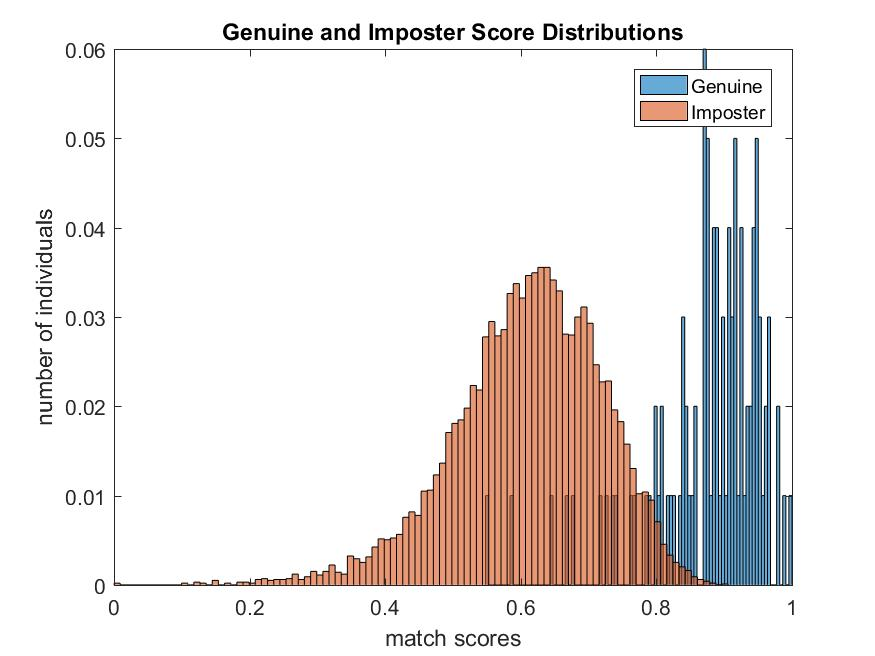
\includegraphics[width=2.4in]{Part1Dis.jpg}
	\caption{(a)The genuine and imposter score distributions.}
	\label{scoDis1}
	\end{minipage}
	\begin{minipage}[t]{0.3\linewidth}
	\centering
	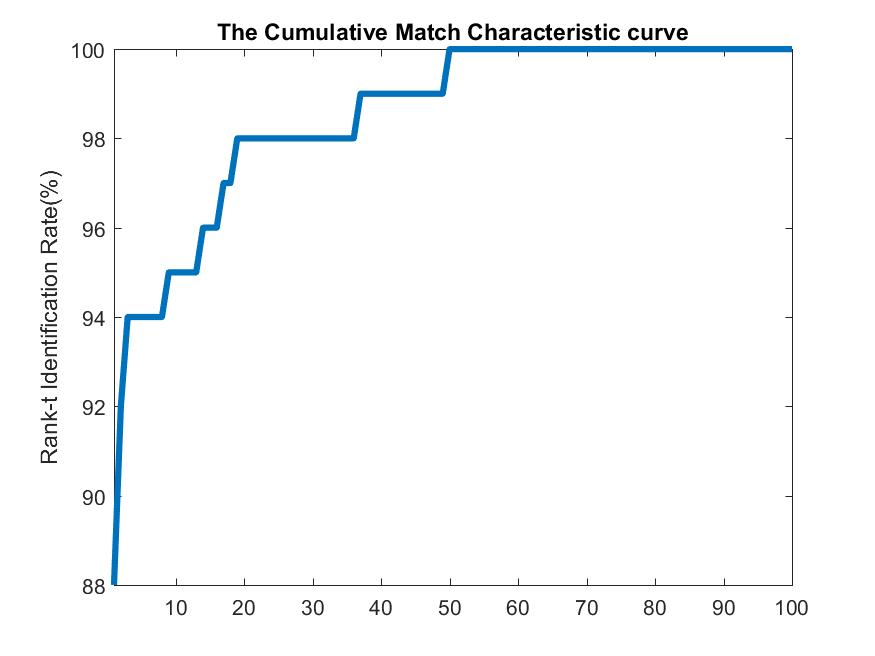
\includegraphics[width=2.4in]{Part1CMC.jpg}
	\caption{(b)The Cumulative Match Characteristic curve.}
	\label{CMC1}
	\end{minipage}
	\begin{minipage}[t]{0.3\linewidth}
	\centering
	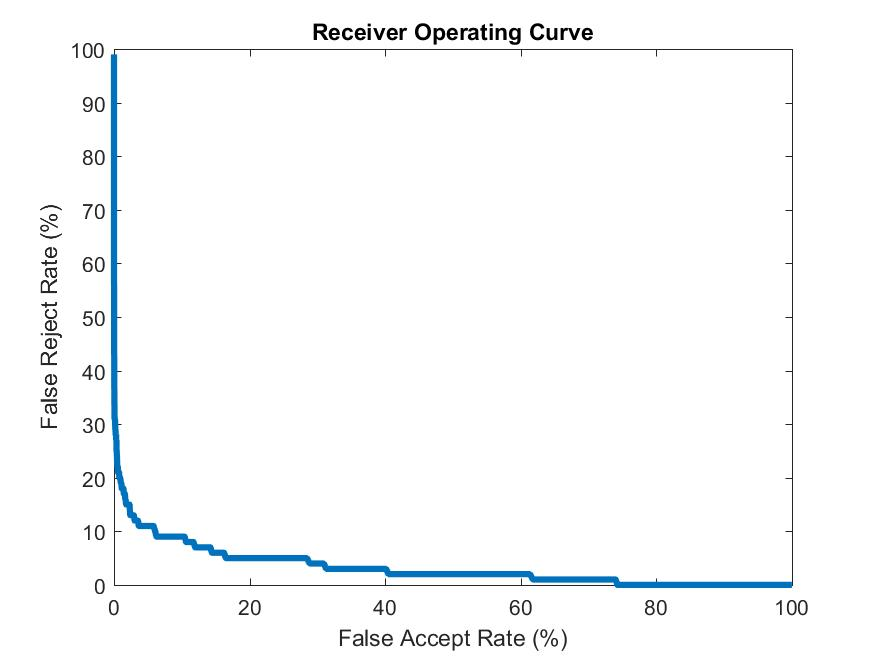
\includegraphics[width=2.4in]{Part1ROC.jpg}
	\caption{(c)The Receiver Operative Characteristic curve.}
	\label{ROC1}
	\end{minipage}
	\end{figure}

	\begin{enumerate}[(a)]
	\setcounter{enumi}{3}
	\item The multi-sample biometric system here is simulated in this way: there are two samples for every individual, for each gallery image, two probe images are matched to and the final results are gained by fusion of either the features of two samples, or the match scores gained from the two samples. Since I am using score level fusion, it is simply take the average of two set of match scores. Note that the match scores are rescaled to range [0,1] already.
	\item I used score level fusion. No score normalization is used, since both of the scores come from the same sensor and same algorithm. Sum rule was used. But the final combined score is normalized (rescaled) to the range [0,1] using min-max rule.
	\end{enumerate}
	
\section*{\huge\textbf{ Task \uppercase\expandafter{\romannumeral2} Multi-Algorithm Biometric System}  }
	\normalsize
	\begin{figure}[H]
	\begin{minipage}[t]{0.3\linewidth}
	\centering
	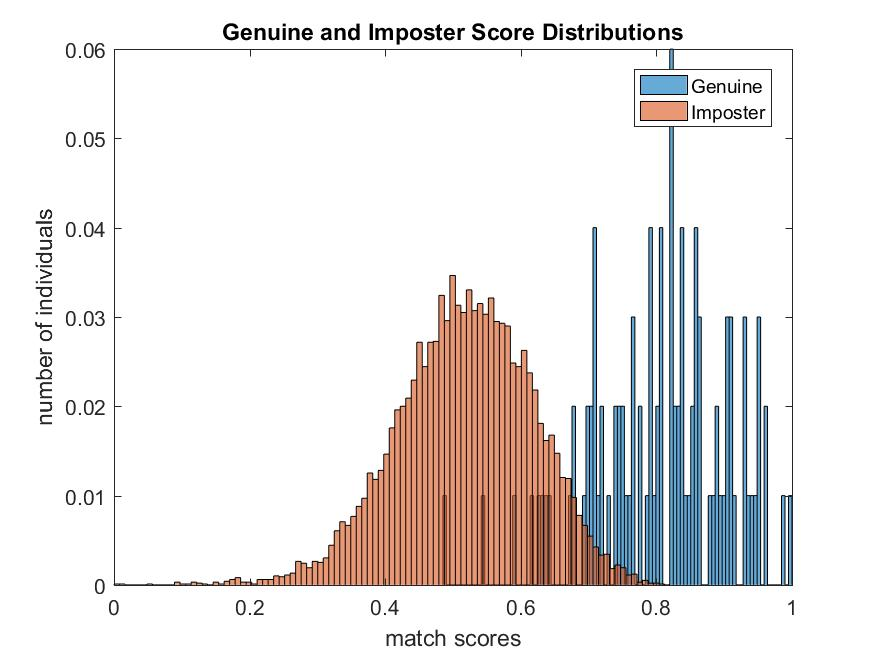
\includegraphics[width=2.4in]{Part2Dis.jpg}
	\caption{(a)The genuine and imposter score distributions.}
	\label{scoDis2}
	\end{minipage}
	\begin{minipage}[t]{0.3\linewidth}
	\centering
	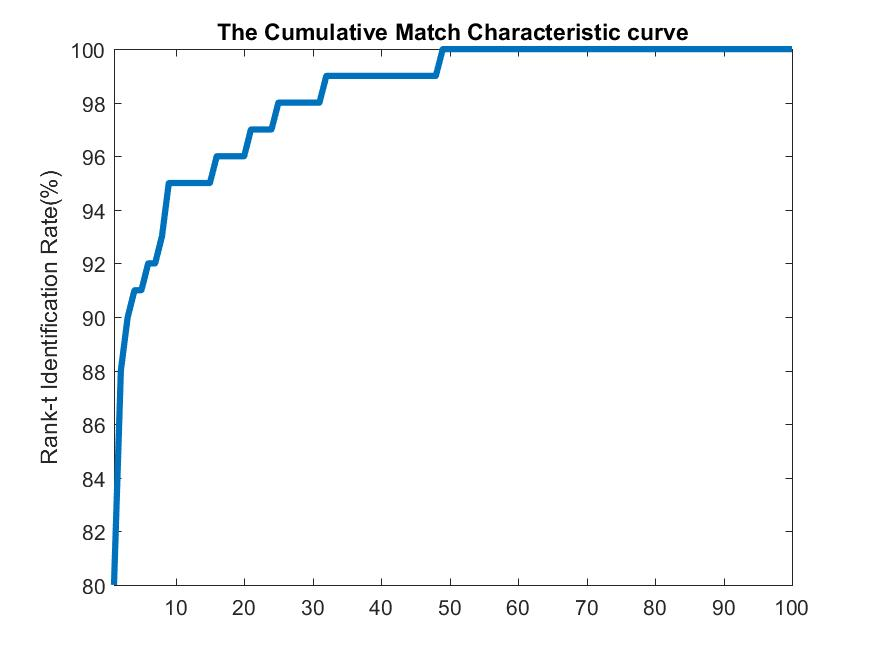
\includegraphics[width=2.4in]{Part2CMC.jpg}
	\caption{(b)The Cumulative Match Characteristic curve.}
	\label{CMC2}
	\end{minipage}
	\begin{minipage}[t]{0.3\linewidth}
	\centering
	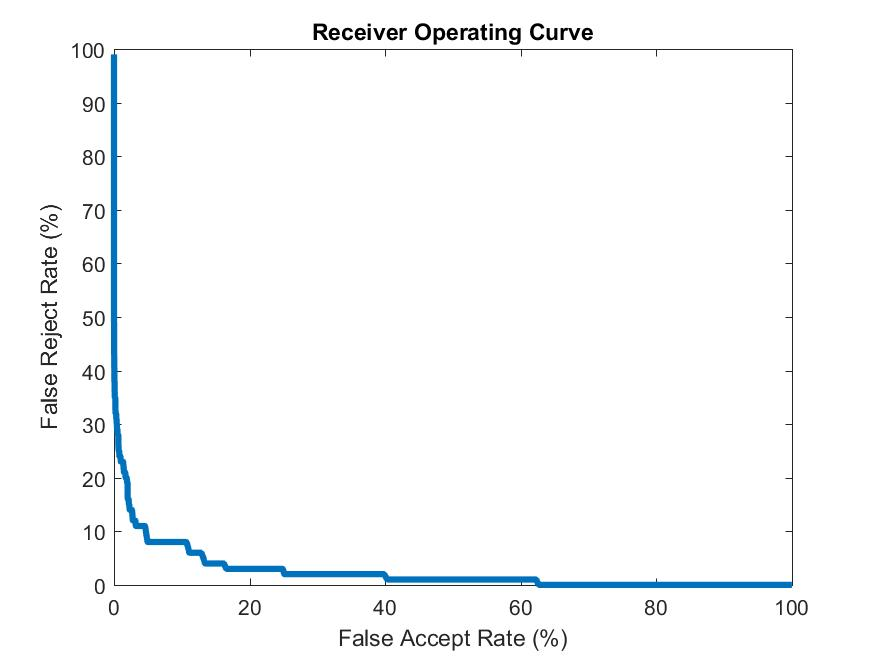
\includegraphics[width=2.4in]{Part2ROC.jpg}
	\caption{(c)The Receiver Operative Characteristic curve.}
	\label{ROC2}
	\end{minipage}
	\end{figure}
	
	\begin{enumerate}[(a)]
	\setcounter{enumi}{3}
	\item The multi-algorithm biometric system is simulated by using only the first probe face image from the data set, with two algorithms of score generation, correlation and PCA. Both the correlation coefficient and the PCA coefficient are rescaled to the range [0,1] before fusion.
	\item I used score level fusion. Min-max normalization is used scores from both algorithms; and what is more, since the correlation coefficient measures the similarity, while the PCA coefficient measures what is like the distances, (1-PCA coefficient) is used to gain the similarity scores. Sum rule was used.
	\end{enumerate}

\section*{\huge\textbf{ Part \uppercase\expandafter{\romannumeral3} Multi-modal Biometric System}  }
	\normalsize
	\begin{figure}[H]
	\begin{minipage}[t]{0.3\linewidth}
	\centering
	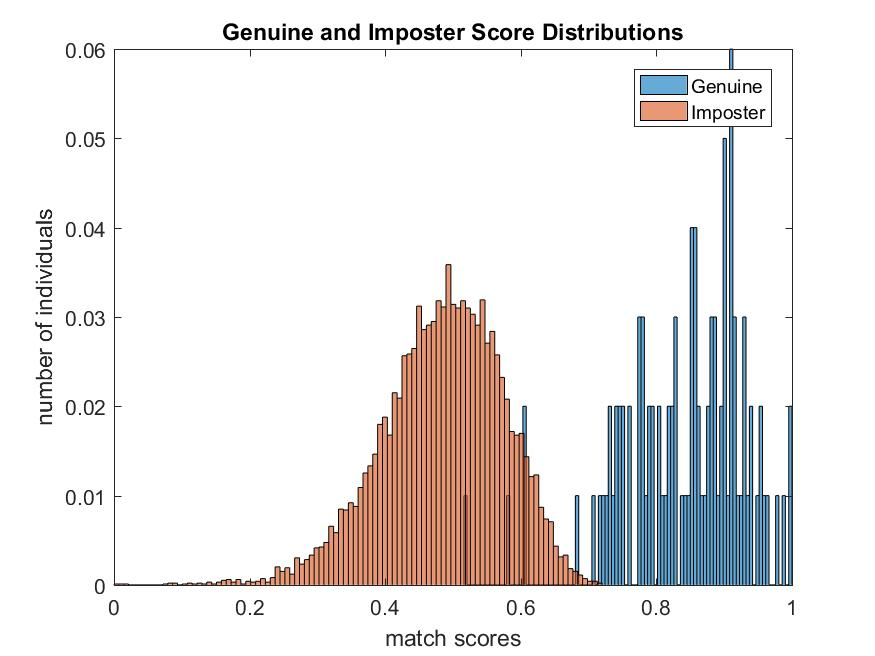
\includegraphics[width=2.4in]{Part3Dis.jpg}
	\caption{(a)The genuine and imposter score distributions.}
	\label{scoDis3}
	\end{minipage}
	\begin{minipage}[t]{0.3\linewidth}
	\centering
	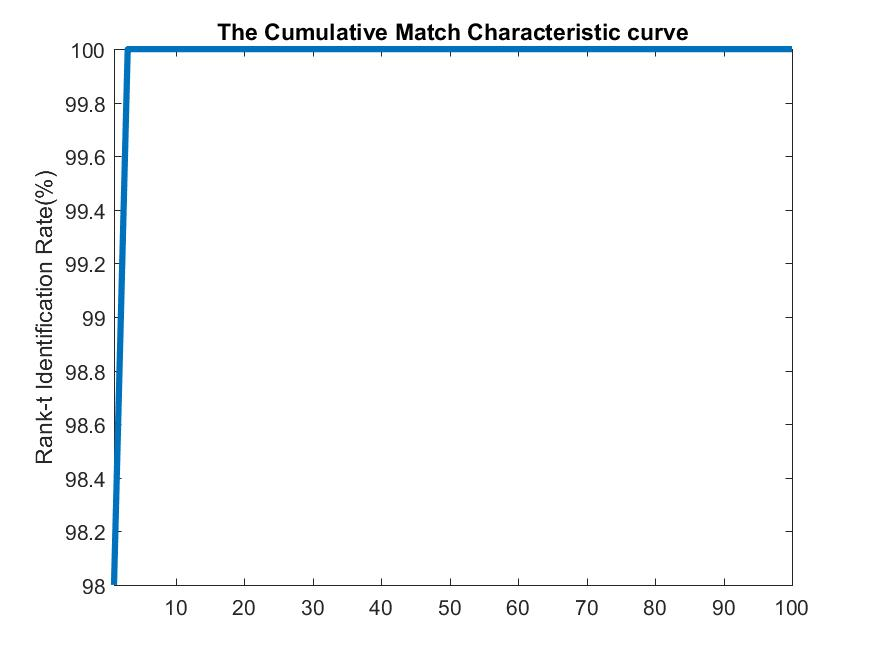
\includegraphics[width=2.4in]{Part3CMC.jpg}
	\caption{(b)The Cumulative Match Characteristic curve.}
	\label{CMC3}
	\end{minipage}
	\begin{minipage}[t]{0.3\linewidth}
	\centering
	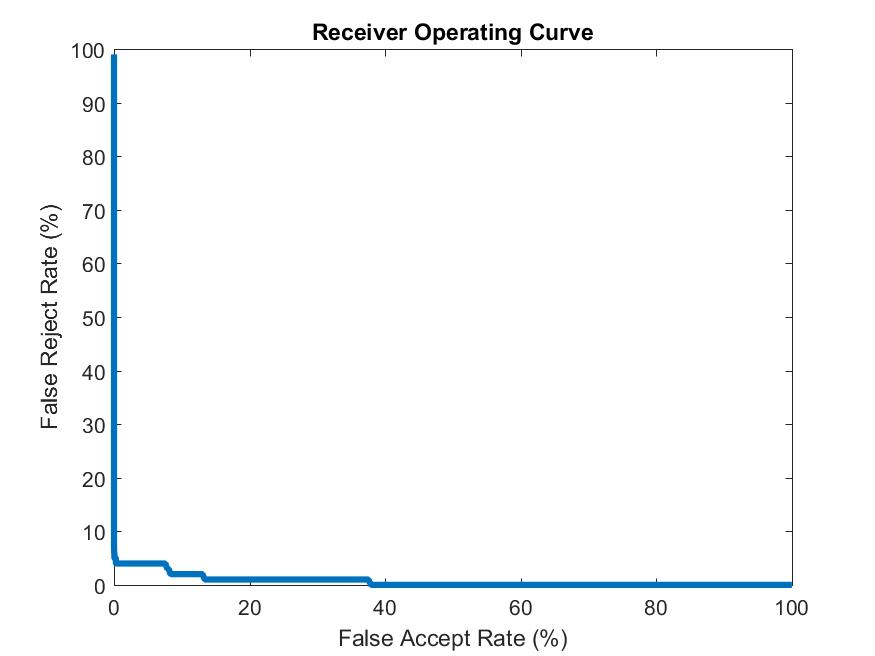
\includegraphics[width=2.4in]{Part3ROC.jpg}
	\caption{(c)The Receiver Operative Characteristic curve.}
	\label{ROC3}
	\end{minipage}
	\end{figure}
	
	\begin{enumerate}[(a)]
	\setcounter{enumi}{3}
	\item The multi-modal biometric system is simulated by using only the first probe face image from the data set and the iris probe image, the gain there match scores separately, where the match scores for face recognition is the correlation coefficient, while the match scores for iris recognition is calculated by Hamming distance. The model is built by fusion these two sets of scores.
	\item I used score level fusion. Min-max normalization is used scores from both algorithms; and what is more, since the correlation coefficient measures the similarity, while the PCA coefficient measures what is like the distances, (1-PCA coefficient) is used to gain the similarity scores. Sum rule was used.
	\end{enumerate}

\section*{\huge\textbf{ EXTRA CREDIT: Non-Ideal Samples}  }
	\normalsize  Prior to extracting features from the iris probe image, smooth the images using a $5\times 5$ mean filter. Use only the bottom half of the first face probe image for feature extraction. The corresponding results are shown below:
	\begin{figure}[H]
	\begin{minipage}[t]{0.3\linewidth}
	\centering
	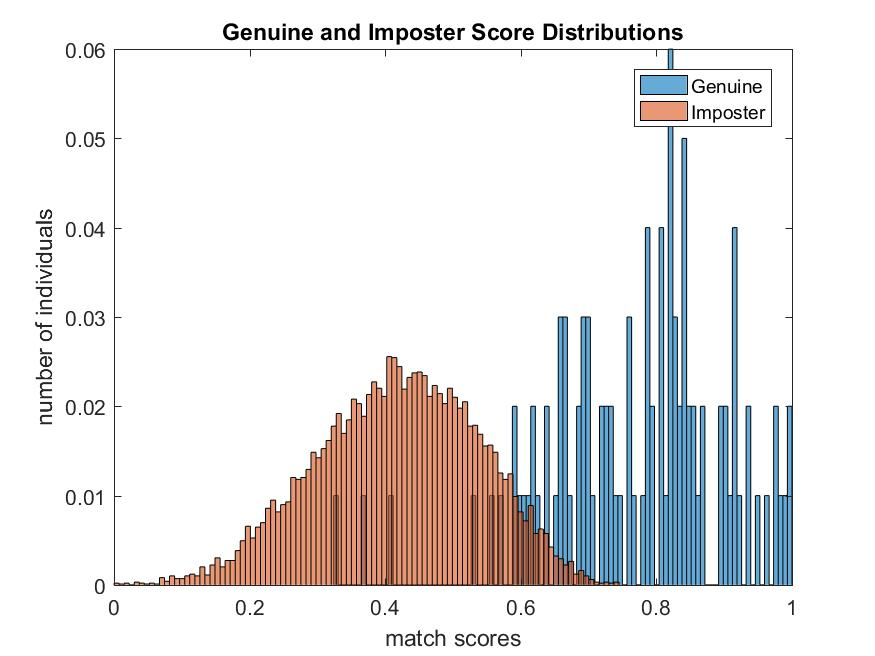
\includegraphics[width=2.4in]{PartExtra3Dis.jpg}
	\caption{(a)The genuine and imposter score distributions.}
	\label{scoDis3}
	\end{minipage}
	\begin{minipage}[t]{0.3\linewidth}
	\centering
	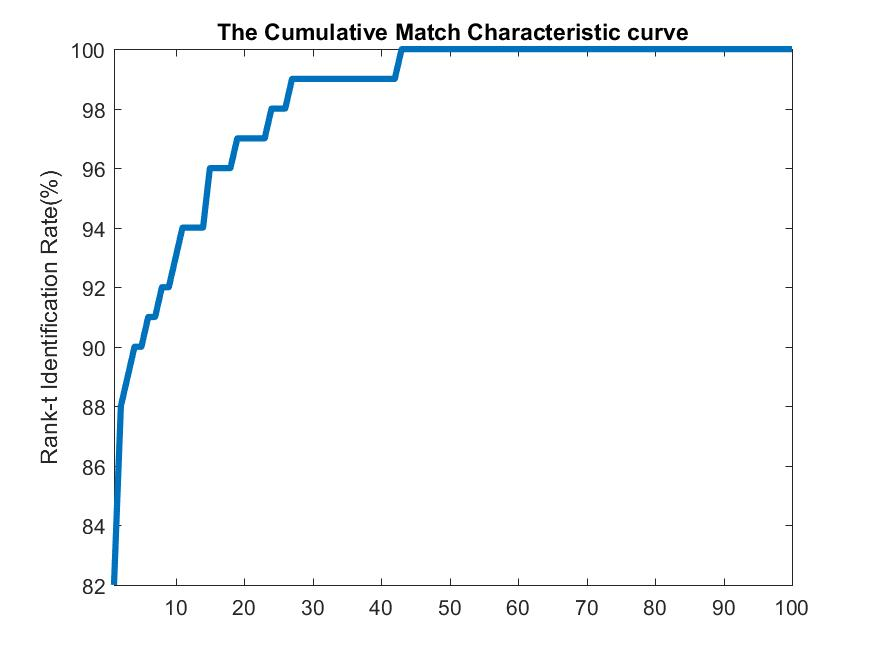
\includegraphics[width=2.4in]{PartExtra3CMC.jpg}
	\caption{(b)The Cumulative Match Characteristic curve.}
	\label{CMC3}
	\end{minipage}
	\begin{minipage}[t]{0.3\linewidth}
	\centering
	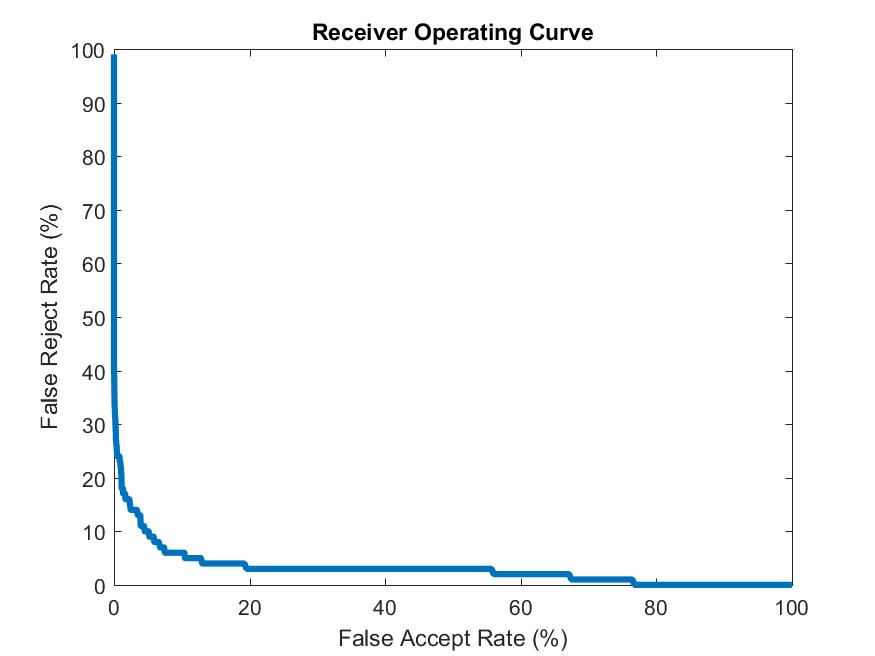
\includegraphics[width=2.4in]{PartExtra3ROC.jpg}
	\caption{(c)The Receiver Operative Characteristic curve.}
	\label{ROC3}
	\end{minipage}
	\end{figure}
	
	\begin{enumerate}[(a)]
	\setcounter{enumi}{4}
	\item Same as what have been done above, I used score level fusion. Min-max normalization is used scores from both algorithms; and what is more, since the correlation coefficient measures the similarity, while the PCA coefficient measures what is like the distances, (1-PCA coefficient) is used to gain the similarity scores. Sum rule was used.
	\end{enumerate}
	
	\noindent Compare to the previous system discussed in part \uppercase\expandafter{\romannumeral3}, where the entire face images as well as non-smoothed iris images are used to extract the features, I would conclude that the sample quality would cause the performance become poorer.\\
	Compare to the previous system discussed in part \uppercase\expandafter{\romannumeral1} and part \uppercase\expandafter{\romannumeral3}, where in the forcer situation only face is used, while in the latter case, both face and iris are used, we can clearly conclude that the using multi-modal system would improve the performance.\\
	When compare the multi-modal with non-ideal samples and the single-modal system, no obvious improving is observed. \\
	To conclude, in a multi-modal system, to improve the performance, the quality of samples is of importance. Multi-modal systems are normally expensive than single-modal systems, but with non-ideal samples, the improvement of performance would not be obvious with higher costs. 

	
	


	
\end{spacing}
\end{document}